% READ ME, PLEASE !!!!
% This document is based on the LaTeX format of Mark T. McLaughlin's thesis
% which was made with WinEdt 5.4, October 2005.  This top section is his
% comments.
%
% 1) IF YOU CAN'T FORMAT SOME PART OF YOUR THESIS ACCORDING TO THE CSULB
%    THESIS GUIDELINES:   DON'T WORRY!!
%    Just rewrite the crap in MSWord. The command, \usepackage{times}
%    puts everything in the same font as the times roman used by MSWord
%
% 2) There are a few SMALL PROBLEMS with the
%    table of contents, list of figures, and list of tables. The problems are
%    a) appendix subhead titles are not supposed to be included in the table of
%    contents, b) figures in the appendices are not supposed to be included
%    in the list of figures, and c) tables in the appendices are not supposed to be
%    included in the list of tables. -EASY SOLUTION: Make up a phony appendix, say
%    phonyAppendixA, which is blank, but the same number of pages as your real
%    appendix A. (Similarly, do the same with appendix B, appendix C, etc...)
%    Then at the end of this file, main.tex, comment out your real
%    appendix A, and uncomment this phony appendix when you LaTex your document
%    for the purposes of generating a table of contents, list of figures, and
%    list of tables. Then when you want to LaTex the rest of your real document,
%    comment out your phony appendices, and uncomment your real appendices.
%
% Everything else passed the thesis office inspection!!! -Bibliography, Signature page,
% Equation numbering, figures, tables, margins, all that junk......
% Thanks Yamato Matsuoka for creating such a nice thesis template!
%
% MORE HELPFUL STUFF:
% TIPS FOR MAKING FIGURES AND TABLES
%   AUTOCAD:
%       In Windows: autocad -> HP color laserjet postscript -> print to filename.ps
%       In Linux: pstoedit -f xfig filename.ps filename.fig
%                 xfig filename.fig
%        in xfig: export -> filename.eps
%        put filename.eps in LaTex document
%
%   EXCEL: excel -> print to postscript (in printer settings click on eps postscript)
%       In Linux: pstoedit -f xfig filename.ps filename.fig
%        in xfig: export -> filename.eps
%        put filename.eps in LaTex document
%

%% =====================================================================
%% Thesis --- Main LaTeX File  ver 0.1
%%                 Date: 6/22/2011 started
%% =====================================================================

\documentclass[12pt]{csulb_thesis}
%\documentclass[12pt]{report}  %% regularly use this
\usepackage{amsmath}   %% mainly to use align environment
\usepackage{amssymb}   %% to use \boldsymbol
\usepackage{times}
%\usepackage{txfonts}
%%% txfonts converts default CM fonts to the followings
%%  Computer Modern Roman      -->  Times
%%  Computer Modern San Serif  -->  Helvetica
%%  Computer Modern Typewriter -->  Corresponding Typewriter Font


%\usepackage[dvipdfm]{color}  %% if you like

%\usepackage[dvips]{graphicx}
% \usepackage[dvipdfm]{graphicx}
\usepackage{graphicx}
\usepackage{hyperref}

%% For printing use   [Option `hyperref.sty' is needed]
\hypersetup{colorlinks=false}

% -------------
% For pdfLaTeX
%\usepackage[pdftex]{graphicx,color}
%\usepackage[pdftex,colorlinks]{hyperref}
% -------------

%%
%\allowdisplaybreaks[1]
%%% \allowdisplaybreaks[n] ... allow pagebreak within eqnarray/align environment n = 1~4

\nonstopmode  % Keep compiling even when errors occur


%% ----------------------------------
%%            Newcommands          %%
% \newcommand{\vect}[1]{\boldsymbol{#1}}  % vector (bold symbol)
% \newcommand{\uvec}[1]{\hat{\vect{#1}}}  % unit vector (bold & hat)
% \newcommand{\mytxt}[1]{\texttt{#1}}
% \newcommand{\mybold}[1]{\textbf{#1}}
% \newcommand{\prof}[1]{Dr$.$ {#1}}
% \newcommand{\myA}[1]{A$({#1})$} %A(t), the acoustic signal from the microphone
% \newcommand{\myB}[1]{B$({#1})$} %B(t), a signal N times the freq of A(t)
\newcommand{\tab}{\hspace*{1.5em}}

%% ----------------------------------


%% ----------------------------------
%%          Author's Info          %%
\title{Problems with Crossover Bias for Binary String Representations in Genetic Algorithms}
\author{Brian Cleary}
\gradmonth{August }  % month & year of the graduation
\gradyear{2011}  % month & year of the graduation
\department{Department of Computer Science and Computer Engineering} % department
\degree{Master of Science} % CSULB degree
\bachelor{B.S.}  % bachelor degree (abbreviated)
\bacheloryear{2003}  % The year bachelor degree was given
\undergraduniv{California State University, Long Beach} % university where the degree was earned
%% ----------------------------------



%% ---------------------------------%%
%%       Thesis Committee           %%
\firstmember{Shui-Fung Lam, Ph.D. (Chair)} %%% Don't forget to put (Chair) at last
\deptfirst{Computer Science}

\secondmember{Kenneth James, Ph.D.} 
\deptsecond{Computer Science}

\thirdmember{Burkhard Englert, Ph.D.} 
\deptthird{Computer Science}

\deanname{Kenneth James, Ph.D.} 
\deandept{Department Chair, Computer Science}
%% ----------------------------------


%%------------- Begin Document -------------------%%
%%                                                %%
\begin{document}
\abstract{\thispagestyle{empty}

Genetic algorithms, a popular technique for optimization, traditionally uses binary pressure will be applied to make up for the bias against some values.  }
\maketitle

%\pagenumbering{arabic} %%%%%%% Comment Out if the abstract is one page long %%%%%%%%%%
%\pagestyle{empty}     %%%%%%% Uncomment   if the abstract is one page long %%%%%%%%%%


%%%---- Insert them if \signaturepage is not used ----
%\pagenumbering{roman}
%\setcounter{page}{2}   %%% Adjustment of Page numbering
%%%----

\signaturepage
% \include{acknowledgement}
\tableofcontents 
\listoffigures
\listoftables

%%%%%%%%%%%%%%%%%%%%%%%%%%%%%%%%%%%%%%%%%%%%%%%%%%%%
%%    This is manually inserted TOC entry!        %%
\addtocontents{toc}{\protect\contentsline{chapterhead}{\chaptername}{}{}}
%% the last {} may be removed if `hyperref.sty' is NOT used.
%%%%%%%%%%%%%%%%%%%%%%%%%%%%%%%%%%%%%%%%%%%%%%%%%%%%

%%%% Similarly, the following should be inserted somewhere in the document
%%%%%%%%%%%%%% TOC entry ! %%%%%%%%%%%%%%%%%%%%%
%%\addtocontents{toc}{\protect\contentsline{chapterhead}{\chaptername}{Page}{}}
%%%%%%%%%%%%%%%%%%%%%%%%%%%%%%%%%%%%%%%%%%%%%%%%

%%%% Or, insert the following if page breaking occurs in appendix entries
%%%%%%%%%%%%%% TOC entry ! %%%%%%%%%%%%%%%%%%%%%
%%\addtocontents{toc}{\protect\contentsline{chapterhead}{\null}{Page}{}}
%%%%%%%%%%%%%%%%%%%%%%%%%%%%%%%%%%%%%%%%%%%%%%%%


\clearpage \pagenumbering{arabic}
\chapter{Introduction}\label{ch:introduction}
\section{Optimization}

Improvement means finding better solutions to problems.  These problems may be to win a game \cite{re:mri}\cite{re:lightbot}.  Any system for which the quality of a  function.\footnote{Some objective functions make the goal minimization rather than maximization, but the process is effectively the same.}  Some situations require  method is the Genetic Algorithm, the subject of this work.  

The simplest optimization method is to examine every solution in the search space, to compute, time is often given in iterations rather than seconds.

\subsection{Mastermind}
Consider a simple code-breaking game to be referred to henceforth as Mastermind \cite{re:mastermind}.  The objective of the player is to guess a multi-digit sort of difficult problem for which approximate optimization is often used \cite{re:knuth}\cite{re:stuckman}.

The objective function is defined in equation 1.  The motivation behind it will be explained in section~\ref{sec:evolutionaryheuristics}.
	\begin{equation}
		\label{eq:mastermindfitness}
		f(code) = correct + log(partially correct)
	\end{equation}

\subsection{Random Search}
Another obvious optimization method would be to repeatedly guess while keeping probability of having found the optimum in $k$ trials given a search space of size $n$ given by the following equation and shown for various values of $n$ in Figure~\ref{fig:randomsearchprobability}.  
 
	\begin{equation}
		p(k|n) = 1 - \left(1 - \frac{1}{n}\right)^k
	\end{equation}
	
Given the probability of guessing the solution in $n$ trials is approximately 63\%the objective function for random search is shown in Figure~\ref{fig:randomsearchquality}, normalized to 1 for the maximum possible value.  This shows that, while 

	
	\begin{figure}
		\begin{center}
			\scalebox{0.7}{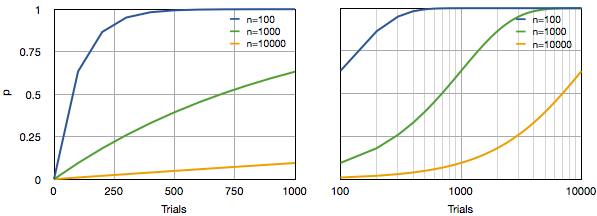
\includegraphics{RandomSearchProbability}} 
		\end{center}
	\caption{Probability of having guessed optimal solution in $k$ trials given search size $n$, for $n$=100, 1000, and 10000.}
	\label{fig:randomsearchprobability}
	\end{figure}

	\begin{figure}
		\begin{center}
			\scalebox{0.80}{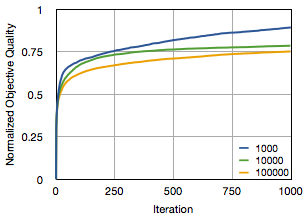
\includegraphics{RandomSearchQuality}} 
		\end{center}
	\caption{Normalized objective function quality for random search of Mastermind for $k$ iterations given search size $n$=100, 1000, 10000.  Averaged over 1000 trials.}
	\label{fig:randomsearchquality}
	\end{figure}

Most evolutionary algorithms include notions of a population, a fitness function, a selection method, and a breeding method \cite{re:evolutionaryalgorithms}.  The population contains potential solutions to an optimization problem, the quality of which is judged by the fitness function.  A generic evolutionary algorithm is shown in Table~\ref{tab:genericevultionaryalgorithm}.

	\begin{table}
		\caption{Generic Evolutionary Algorithm} \hline
		\label{tab:genericevultionaryalgorithm}
		% \begin{tabular}{0.75\textwidth}{l}
		\begin{tabular}{l} \\
		population \(\gets\) random initial values \\ \\
		WHILE fitness of best population member \(\leq\) required fitness \\ \\
			\tab new\_population \(\gets\) empty list\\ \\
			\tab REPEAT \\ \\
				\tab \tab Select parents from the population proportionally to fitness \\ \\
				\tab \tab Breed parents to create children. \\ \\
				\tab \tab Add children to new\_population. \\ \\
			\tab UNTIL size(new\_population) == size(population) \\ \\
			\tab population \(\gets\) new\_population \\
		\end{tabular}
		\hline
	\end{table}
	

A more specific version of evolution is genetic evolution, which treats the gene as the main element of evolution rather than the organism \cite{re:selfishgene}.  of genes, and the breeding methods should be akin to genetic crossover and mutation.  

\subsection{Heuristics} \label{sec:evolutionaryheuristics}
A major way in which algorithms, including optimization methods, can be improved is by designing it to take advantage of knowledge and assumptions made by its 


\chapter{Overview of Genetic Algorithms}
One of the most direct imitations of genetic evolution used for optimization is the 

\section{Genetic Algorithms Operations and Their Purposes}
\subsection{Parts of the Genetic Algorithm}
The main part of the genetic algorithm is the gene, which is a problem parameter 
\chapter{Complications of Genetic Algorithms}
The many variations in genetic algorithms have been created to address numerous genetic algorithm effectiveness.

\section{Diversity}
One of the most fundamental problems that can occur in a genetic algorithm is the probability between 0.01 and 0.001 per bit, the delay would have a high expected duration \cite{re:mutationrate1}\cite{re:mutationrate2}.  For this reason, some on a diversity measure of the population, raising it when the diversity becomes too low.

Another issue of low genetic diversity in the population is that it represents poor Hamming distance between the chromosomes selected for breeding \cite{re:diversityincrossover}.  Conversely, when it is desirable to explore multiple local optima, the same measure could be used to promote crossover within these niches and even partition the population for separate parallel exploration \cite{re:parallelGAniche}.

similar integer values often have very dissimilar binary representations, as shown in Equation~\ref{eq:linearvsHammingdistance} by the linear distance Hamming distance for the integers seven and eight.  If the schemata being explored were $x111_2$ and the optimum value for the problem happened to be $1000_2$, the space worse for a larger pair of values such as $1000000000000000_2$ and $0111111111111111_2$.

	\begin{equation}
		\label{eq:linearvsHammingdistance}
		|7 - 8| = 1 \tab \neq \tab ||0111_2-1000_2||_1 = 4
	\end{equation}

representations.  $1101_2$ and $1100_2$ are close together by both linear and would be useless since no schema would have any approximate meaning.
\chapter{Problems with Combinatorial Crossover Bias for Binary String Genetic Representations}
\section{Distribution of Features and Values}
When using a limited range of integer values, crossover as the recombination of 

% Tony's table edits:
\begin{table}
\caption{Crossover Outcomes for the Range 0 to 2}
\label{tab:crossoveroutcomes0to2}
\begin{center}
\begin{tabular}{ccc}
\hline\\[-0.75pc]
	$00_2 \times 00_2 & \rightarrow &  00_2 \:,\: 00_2$ \\ \\		%\\[0.5pc]
% \hline\\[-0.75pc]
	$00_2 \times 01_2 & \rightarrow &  01_2 \:,\: 01_2$ \\ \\
% \hline\\[-0.75pc]
	$00_2 \times 10_2 & \rightarrow &  10_2 \:,\: 00_2$ \\ \\
% \hline\\[-0.75pc]
	$01_2 \times 00_2 & \rightarrow &  00_2 \:,\: 01_2$ \\ \\
% \hline\\[-0.75pc]
	$01_2 \times 01_2 & \rightarrow &  01_2 \:,\: 01_2$ \\ \\
% \hline\\[-0.75pc]
	$01_2 \times 10_2 & \rightarrow &  00_2 \:,\: 11_2$ \\ \\
% \hline\\[-0.75pc]
	$10_2 \times 00_2 & \rightarrow &  10_2 \:,\: 00_2$ \\ \\
% \hline\\[-0.75pc]
	$10_2 \times 01_2 & \rightarrow &  11_2 \:,\: 00_2$ \\ \\
% \hline\\[-0.75pc]
	$10_2 \times 10_2 & \rightarrow &  10_2 \:,\: 10_2$ \\ 
\hline
\end{tabular}
\end{center}
\end{table}
%
\begin{table}
\caption{Crossover Outcomes Frequency for the Range 0 to 2}
\label{tab:crossoveroutcomefrequency0to2}
\begin{center}
	\begin{tabular}{lcccc}
		\hline \\[-0.75pc]
		Outcome	&	$00_2$	&	$01_2$	&	$10_2$	&	$11_2$	 \\[0.75pc]
		\hline \\[-0.75pc]
		Frequency&	7			&	5			&	4			&	2			 \\[0.5pc]
		\hline\\[-0.75pc]
	\end{tabular}
\end{center}
\end{table}
%



\section{Similarity Problems with Categorical Variables}
As noted previously, another problem with the binary string representation is that 
\chapter{Methodology}\label{ch:methodology}
This work has two main components.  First, demonstrating the existence of the 


\section{Measuring Bias}
\subsection{Measuring the Bias of a Base Set}
The first bias to be measured was that of the base set from which samples will be 
\chapter{Results}\label{ch:results}
\section{Integer Range Bias}
\subsection{Versus offset}
As previously mentioned, it was found that most ranges can be shifted to a lower 
\chapter{Conclusions}

\section{Crossover Bias is Significant}
Combinatorial crossover bias is a significant issue with binary strings.  Crossover that of the form $0..2^n -1$, which includes all normal integer type variables that are some whole number of bytes.

\section{Offset Improvement Significant but Insufficient}
Simple linear offsets make significant but insufficient improvement to the Pearson's $\chi^2$ test for uniformity, almost all would not.  





% \appendix
%\include{phonyAppendixA} %-Use this to make a thesis office approved TOC, LOF, and LOT
%\include{phonyAppendixB} %-Use this to make a thesis office approved TOC, LOF, and LOT
% \include{detailedDescriptionOfTheCircuit}
% \include{circuitConstruction}

%\bibliographystyle{utphys}  % With journal title
% \bibliographystyle{h-physrev} % No journal title appears
% \bibliography{papers}
\begin{thebibliography}{9} %set to single digit for no columnation, two digits for columnation upto [99], etc.
% use style guide: IEEE Computer Society Style Guide


% Introduction
\bibitem{re:mri} %report
J. Rouet et al., ``Genetic algorithms for a robust 3-D MR-CT registration,'' in \textit{IEEE Trans. Inf. Technol. Biomed.}, 2000, vol. 4, pp. 126-136.
% @article{
% author = {Jean-michel Rouet and Jean-josé Jacq and Christian Roux},
% title = {Genetic algorithms for a robust 3-D MR-CT registration},
% journal = {IEEE Transactions on Information Technology in Biomedicine},
% volume = {4},
% year = {2000},
% pages = {126--136},
% doi = {10.1109/4233.845205},
% masid = {801806}
% }

\bibitem{re:lightbot} %electronic
% http://gfredericks.com/sandbox/light_bot
G. Fredericks, \textit{Light-Bot Genetic Algorithms,} 2011, June 16;   http://gfredericks.com/sandbox/light\_bot 
% @Electronic{ re:lightbot,
%   author    = "Gary Fredericks",
%   title     = "Light-Bot Genetic Algorithms",
%   url       = "http://gfredericks.com/sandbox/light_bot",
%   month     = jun,
%   year      = "2011",
% }

\bibitem{re:mastermind} %electronic
E. W. Weisstein, \textit{Mastermind,} 2011, June 16; http://mathworld.\\wolfram.com/Mastermind.html


\bibitem{re:knuth} %report/article
% Knuth, Donald (1976-77), "The Computer as a Master Mind," J. Recr. Math. (9): 1–6
D. Knuth, ``The Computer as a Master Mind'', \textit{J. Recr. Math.}, 1976, vol. 9, pp. 1–6.

\bibitem{re:stuckman} %report/article
% @article{DBLP:journals/corr/abs-cs-0512049,
%   author    = {Jeff Stuckman and
%                Guo-Qiang Zhang},
%   title     = {Mastermind is NP-Complete},
%   journal   = {INFOCOMP Journal of Computer Science}
%   volume    = {5},
%   year      = {2006},
		% pages = {25--28},
%   ee        = {http://arxiv.org/abs/cs/0512049},
%   bibsource = {DBLP, http://dblp.uni-trier.de}
% }
J. Stuckman and G. Zhang, ``Mastermind in NP-Complete,'' in \textit{INFOCOMP J. Comput. Sci.}, 2006, vol. 5, pp. 25-28.

\bibitem{re:simulatedannealing}  %report/article
% Kirkpatrick, S.; Gelatt, C. D.; Vecchi, M. P. (1983). "Optimization by Simulated Annealing". Science 220 (4598): 671–680.
S. Kirkpatrick et al., ``Optimization by Simulated Annealing,'' in \textit{Science}, 1983, vol. 220, Issue 4598, pp. 671-680.

\bibitem{re:antcolony} %book
 % Swarm intelligence book pp 105-109
J. Kennedy et al., \textit{Swarm Intelligence}, Morgan Kaufmann Publishers, 2001, pp. 105-109.
% @book{kennedy2001swarm,
%   title={Swarm intelligence},
%   author={Kennedy, J. and Eberhart, R.C. and Shi, Y.},
%   isbn={9781558605954},
%   lccn={00069641},
%   series={The Morgan Kaufmann series in evolutionary computation},
%   url={http://books.google.com/books?id=vOx-QV3sRQsC},
%   year={2001},
%   publisher={Morgan Kaufmann Publishers}
% }

\bibitem{re:originofspecies} %book
% sponge's book p 31-51 
D. B. Fogel, \textit{Evolutionary Computation: Toward a New Philosophy of Machine Intelligence}, 2nd ed., IEEE Press, 2000, pp. 31-51.

\bibitem{re:evolutionaryalgorithms} % swarm book pp 133-186
J. Kennedy et al., \textit{Swarm Intelligence}, Morgan Kaufmann Publishers, 2001, pp. 133-186.


\bibitem{re:selfishgene} %book
% dawkins pp 46-65
R. Dawkins, \textit{The Selfish Gene}, 30th Anniversary ed., Oxford University Press Inc., 1976, pp. 46-65.  

% Overview
\bibitem{re:mutationrate1} %report/article
% DeJong, K.A. and Spears, W.M. "An Analysis of the Interacting Roles of Population Size and Crossover in Genetic Algorithms," Proc. First Workshop Parallel Problem Solving from Nature, Springer-Verlag, Berlin, 1990. pp. 38-47.
K. A. DeJong and W. M. Spears, ``An Analysis of the Interacting Roles of Population Size and Crossover in Genetic Algorithms,'' in \textit{Proc. 1st Workshop Parallel Problem Solving from Nature}, Springer-Verlag, 1990, pp. 38-47.


\bibitem{re:mutationrate2} %report/article
% Grefenstette, J.J. "Optimization of Control Parameters for Genetic Algorithms," IEEE Trans. Systems, Man, and Cybernetics, vol. SMC-16, no. 1, Jan./Feb. 1986, pp. 122-128.
J. J. Grefenstette, ``Optimization of Control Parameters for Genetic Algorithms,'' in \textit{IIEEE Trans. Syst. Man Cybern.}, vol. SMC-16, no. 1, Jan./Feb. 1986, pp. 122-128.

% \bibitem{populationboiling} %

\bibitem{re:diversityincrossover} %report/article/chapter
% @inproceedings{
% author = {Larry Eshelman},
% title = {The CHC Adaptive Search Algo-rithm},
% booktitle = {Foundations of Genetic Algorithms},
% year = {1991},
% masid = {3866190}
% }
L. Eshelman, ``The CHC Adaptive Search Algorithm,'' in \textit{Foundations of Genetic Algorithms}, G. J. E. Rawlins, ed., Morgan Kaufmann Publishers Inc., 1991, pp. 265-283.


\bibitem{re:schema} %book
J. Holland, \textit{Adaptation in Natural and Artificial Systems}, University of Michigan Press, 1975.


% Complications 

\bibitem{re:parallelGAniche} %thesis
S. Mahfoud, ``Niching Methods for Genetic Algorithms,'' Ph.D. dissertation, Dept. General Eng., Univ. Illinois, Urbana-Champaign, 1995.

\bibitem{re:nfl} %report/article
D. H. Wolpert and W. G. Macready, ``No Free Lunch Theorems for Optimization,'' in \textit{IEEE Trans. Evol. Comput.}, vol. 1, no. 67, April 1997.

% Methodology
\bibitem{re:pearson} %report/article
R. L. Plackett, ``Karl Pearson and the Chi-Squared Test,'' in \textit{International Statistical Review / Revue Internationale de Statistique}, vol. 51, no. 1, Apr. 1983, pp. 59-72.
% @Article{ re:pearson,
%   author    = "R. L. Plackett",
%   title     = "Karl Pearson and the Chi-Squared Test",
%   journal   = "International Statistical Review / Revue Internationale de StatistiqueNumerische Mathematik",
%   volume    = "51", 
%   number		= "1",
%   pages     = "59-72",
%   month		= "April",
%   year      = "1978",
% }
\end{document}
%%                                                            %%
%%------------- End of Document ------------------------------%%
